\section{Group Testing} \label{sec:w12_GT}
\lecture{6 May}

Here we continue on with the discussions on group testing from \autoref{sec:w11_GT}. Let us recap the problem setting: we have $x\in\{0.1\}^{n\times1}$ where $x_i=1$ if and only if the $i$th person is infected, with $m$ being the number of test / measurement. Normally, $k=\norm{x}_0$ is small, for example, $k\sim\sqrt{n}$ or $n^c$ with $c\in[0,1)$, or else the population simply dies out as the disease is so widespread and group testing will be the last of our concerns. Our task is to solve the system of \textit{logical} equations $y=Ax$. One can rewrite this system of logical equations using the usual linear algebra:
\begin{align}
    y^\star &= Ax,\, y^\star_i = \sum_{j}A_{ij}x_j \notag\\
    \Rightarrow y_i &= \min(y^\star_i,1) \\
    \Rightarrow y &= \min(y^\star,\vec{1}),
\end{align}
where $\vec{1}\in\mathbb{R}^{n\times1}$ is the vector of ones.

Besides using the \textit{activation function} $\min(\cdot,1)$, one can opt for arbitrary functions of similar behavior. For example, the ReLU, sigmoid, or $\arctan$ are some suitable replacements. All that is needed is the monotonicity of the activation function. For more information, please refer to the reference \cite{Generalized_Group_Testing}.

\subsection{Applications of Group Testing}
The study of group testing originated from WWI\!I, where it is used to reduce the amount of test required to find out syphilitic males in soldiers. Nowadays, its applications become almost pervasive, appearing in every corner of modern science. Some examples are listed below, with special emphasis put on heavy hitters and bloom filter.

\paragraph{Genotyping:} The task of genotyping is to find out whether you have a certain strand of gene that, for example, may cause cancer. The human DNA consists of around 3 billion base pairs, it is too costly and impossible to test one-by-one whether a sequence of gene appears in the DNA. Instead, we can use group testing to aid our task. Given a solution of one's DNA, we can apply the CRISPR (a DNA scissor technology) to cut the DNA into suitable strands and heat up the solution so that the double helix unwinds. Next, we prepare a bunch of already-known sequences of cancer genes and connect them with probes that are light emitting when the sequences are bound by its complementary sequence. By mixing the cancer gene sequences with the DNA solution, some of them combines and emits light. Our detector captures this light emission and determines whether a cancer gene is present. Due to the noise inherent in the experiment, this is actually a harder problem of noisy group testing.

\paragraph{Unsourced access:} Given $n$ cellphones near a base station with $k$ of them wanting to talk, how does the base station know which phone is talking what? The time-frequency spectrum is cut into different regions in the communication frequency band: each time slot and frequency slot allows for only one phone transmitting their data (with error correcting code of course). A phone sends its signals by \textit{randomly} choosing a slot. Inevitably, collision may occur where two different phones are talking, and the signals they sent become undecodable. How then, can we resolve collisions in a simplest possible way? The result also requires group testing.

\paragraph{Computer forensics:} Imagine having files saved on your computer and a hacker comes along and modified some of them. How do you detect the modification and fix it, or even better, prevent the modification from even happening? The simplest way is to have your computer never connect to the internet, which is impossible for most practical purposes. Instead, one can utilize what is called a \textit{hash function}. A hash function is a special kind of function that is easy to compute, but \textit{very} difficult to invert, viz., $y=\mathrm{hash}(x)$ is easy to compute, $x=\mathrm{hash}^{-1}(y)$ is hard to compute. For each file, we can create their hash values and store it in a separate database -- so that if a file doesn't match its hash value, we know that it is modified. Except that it doesn't, the hash values can also be modified by the hacker, and a document may be regarded as modified even though it is not! Instead of having a hash value for each file separately, we can group multiple files together to form a single hash value. These hash values are stored in a separate computer. Since the data size for the hash values is smaller then the previous case, we can apply a higher security level on these data to make them difficult to be modified. Just like the bipartite graph of \autoref{fig:w11_group_test}, if a file is modified, some of the hash values do not match, and we can use group testing to pinpoint exactly which file is modified.

\paragraph{Image compression:} An image can be compressed or be represented by fewer bits than its na\"ive representation due to the fact that most natural images are sparse in its Fourier domain. Viz., when applying the Fourier transform to a natural image, most of the Fourier coefficients are close to zero and can be omitted. How do we quickly find out the non-zero coefficients? This task, again, can be solved via group testing. For the more educated readers, one might also draw parallel of this task with the research of \textit{compressed sensing} (or compressive sensing). In fact, they are the same! The only difference lies in their choice of the activation function. For generalized group testing, one might use the logarithmic function as an activation function since it mimics the log-scale sensitivity of human perception (in visual and auditory system).

\paragraph{Heavy hitter:} The task of heavy hitter is to find out which elements are more popular, i.e., which YouTuber has the most subscribers, who's videos has the most view count, which computer file is used most often. Take the last one for example: In a server, we have SSD (solid state drive) and HDD (hard disk drive) as hardware disks, the former is faster in its read and write processing but more expensive, while the latter is slower but cheaper. A reasonable setup is to have, for exmaple, 250GB to SSD used as system disk and 4TB of HDD allocated for saving less-commonly used documents or old photos. Our task is to find out, out of all the $n$ files, which of the $k$ ones are the most popular? It should be noted that the probability of a file being used follows the famous \textit{Zipf distribution}\footnote{This distribution appears everywhere!}, hence only a small fraction of files are actually commonly used, and we can order them from the most often-used ones to the least used ones by allocating them to registers, caches, RAM, SSD, then finally HDD. To efficiently count the frequency of each entry, one can use a \textit{bloom filter}, which will be introduced immediately.

\subsection{Bloom Filter}
When registering for an account on a website, one often sees the sentence ``Invalid username, the username is already taken." How does the server immediately knows that a username appears in the database? It seems impossible to check for every single username in the database for repetition on the fly.

And you are absolutely correct, the server indeed does not check the entire database. Instead, it prepares a string of, for example, 200 bits at hand. The string is all-zero initially when there are no accounts in the database. When an account is added, the database computes a few hash values to the username, these hash values are between 1 to 200. If the username ``apple" is registered, the database computes $\mathrm{hash}(0\text{ apple}) = 10$, $\mathrm{hash}(1\text{ apple}) = 3$, and $\mathrm{hash}(2\text{ apple}) = 5$, then it sets the position 10, 3, and 5 of the bit string to 1. The same applies to all usernames created. Then the final string should consist of 0's and 1's. If one register for a username, the server quickly computes the hash values and compare with its bit string. If all the positions corresponding to the hash values are 1 one the bit string, then it is likely that the username is already taken, and the server rejects your registration (see \autoref{fig:w12_bloom_filter} below). This is the task of membership testing. Although this method has no missed detection, false positives are still possible. That is not a problem, however, since the company is the boss, and it gets to decide which usernames are possible and you can't argue with it. There is one thing this na\"ve bloom filter cannot do, that is, it cannot delete accounts.

\begin{figure}[H]
    \centering
    \begin{equation*}\begin{array}{|c|c|c|c|c|c|c|c|c|c|c|c}
        \hline
        0 & 1 & 1 & 0 & 1 & 0 & 1 & 0 & 0 & 1 & 0 & \cdots \\
        \hline
    \end{array}\end{equation*}
    \caption{Bloom filter. Assume two strings ``apple" and ``banana" added. They have hash values of $10$, $3$, $5$, and $2$, $5$, $7$. If one wants to add ``cherry" into the database, we have to check whether its hash values collide with the 1's in the list.}
    \label{fig:w12_bloom_filter}
\end{figure}

\paragraph{Bloom counter:} Unlike the bloom filter, setting the hash value positions of registered usernames to 1 with logical arithmetic; the bloom counter \textit{adds 1} to the string with usual integer arithmetic. However, now the string will be 200 \textit{bytes} long (1 byte = 8 bits). With this small modification, the bloom counter can delete members. Nevertheless, it cannot delete false positives... why would one implement such functionality anyways?

\begin{figure}[H]
    \centering
    \begin{equation*}\begin{array}{|c|c|c|c|c|c|c|c|c|c|c|c}
        \hline
        0 & 1 & 1 & 0 & 2 & 0 & 1 & 0 & 0 & 1 & 0 & \cdots \\
        \hline
    \end{array}\end{equation*}
    \caption{Bloom counter. Having the same settings as \autoref{fig:w12_bloom_filter}.}
    \label{fig:w12_bloom_counter}
\end{figure}

\paragraph{Database summary:} Given a bloom filter, can we quickly summarize who is in the database? The answer is yes! Though up to a small chance of false positives. The simplest approach is to enumerate all possible accounts and check if they are in the database. If the format of the usernames is restricted, then the set of usernames is finite, and the algorithm converges... after a long time. Instead, we can use a bloom filter to quickly summarize the \textit{heavy hitters} in the database. The technique we will introduce now is called the ``count sketch" or the ``min count sketch", some other algorithms like GroTesQuE (group testing quick and efficient) \cite{grotesque_GT}, AC-DC \cite{AC-DC_GT}, SAFFRON \cite{saffron_GT} can also be utilized. We will touch on a few of these methods in a later subsection.

The count sketch method is basically just a bloom counter but with a really nice hash function. Consider having a string of 1000 integers ($\mathbb{Z}^{1000}$), we will now describe the procedure and details of adding an item into the database and summarizing the whole database.
\begin{enumerate}[label=(\arabic*)]
    \item To add ``apple" into the database, turn it into a string of integers, for example, $10010001$. How this string is chosen will be clarified later on.
    \item Find the hash values to ``apple", say we have $\mathrm{hash}(0\text{ apple})=2$ and $\mathrm{hash}(1\text{ apple})=4$.
    \item Add the string $10010001$ to the subarrays with index coinciding with the hash values. See \autoref{fig:w12_database_summary_1}.
    \begin{figure}[H]
        \centering
        \begin{equation*}\begin{array}{|c|c|c|c|c|c}
            \hline
            0\,0\,0\,0\,0\,0\,0\,0 &
            1\,0\,0\,1\,0\,0\,0\,1 &
            0\,0\,0\,0\,0\,0\,0\,0 &
            1\,0\,0\,1\,0\,0\,0\,1 &
            0\,0\,0\,0\,0\,0\,0\,0 &
            \cdots \\
            \hline
        \end{array}\end{equation*}
        \caption{Count sketch: adding an item ``apple" into the database.}
        \label{fig:w12_database_summary_1}
    \end{figure}
    \item Anytime I see ``apple", I add $10010001$ to the above hash-value positions again.
    \item Say we added ``apple" a total of 25 times, and ``banana" a total of 75 times. The string ``banana" is represented by $11001001$, with hash values $4$ and $5$. The fourth subarray should have a value of $100\,75\,0\,25\,75\,0\,0\,100$.
    \item Some other not-so-important entries are added, like ``cherry" 10 times, ``durian" 5 times, and so on. There might also be noise within the data. The final string should have a form similar to \autoref{fig:w12_database_summary_2}.
    \item However, due to the noise present, we cannot immediately find out the heavy hitters. The solution is simple, we can use threholding by, for example, 20.
    \begin{figure}[H]
        \centering
        \begin{align*}
        &\begin{array}{|c|c|c|c|c|c|c}
            \hline
            7\,1\,0\,0\,1\,0\,3\,10 &
            25\,0\,5\,25\,1\,0\,6\,25 &
            0\,3\,0\,3\,1\,0\,0\,10 &
            100\,75\,0\,27\,75\,0\,2\,110 &
            75\,85\,3\,0\,75\,0\,0\,77 &
            \cdots \\
            \hline
        \end{array} \\
        &\downarrow \text{ thresholding by 20} \\
        &\begin{array}{|c|c|c|c|c|c}
            \hline
            0\,0\,0\,0\,0\,0\,0\,0 &
            1\,0\,0\,1\,0\,0\,0\,1 &
            0\,0\,0\,0\,0\,0\,0\,0 &
            1\,1\,0\,1\,1\,0\,0\,1 &
            1\,1\,0\,0\,1\,0\,0\,1 &
            \cdots \\
            \hline
        \end{array}
        \end{align*} 
        \caption{Count sketch: final database followed by thresholding to find the heavy hitters.}
        \label{fig:w12_database_summary_2}
    \end{figure}
    \item The second subarray tells us that ``apple" is a heavy hitter, and the fifth subarray tells us that ``banana" is also a heavy hitter. The fourth subarray, however, is a combination of ``apple" and ``banana", hence it is undecodable. In the case where there is larger noise, we can use error correcting codes (ECC) to set the string representations of ``apple" and ``banana." With ECC used, we can counter with 1 or 2 errors.
\end{enumerate}


\subsection{Binary Search + Group Testing} \label{sec:w12_bin_GT}
The tactics and algorithms for group testing are vast, for further reading, one can refer to the references \cite{CombinatorialGT_SparseRecovery,NoisyNonadaptiveGT,Quickly_Decodable_GT}.

Below, we start our discussion of the na\"ive tactic of binary search. We first separate the population into two halves, then conduct group testing on both halves. Depending on which half being positive on the first round of tests, we continue on with the second round of tests on it. The amount of tests required is of order $O(\log n)$. This scheme is \textit{adaptive}, since one saw the test results before conducting further tests. In practical cases, this means that this scheme takes a longer time to conduct since it requires so many stages, which is not ideal, we aim for single round group testing which is non-adaptive.

The following discussion follows mainly from the work by Wang, Gabrys, and Guruswami \cite{Quickly_Decodable_GT}. A non-adaptive scheme for group testing is by binary search. Any binary search is a binary tree.

\begin{figure}[H]
    \centering
    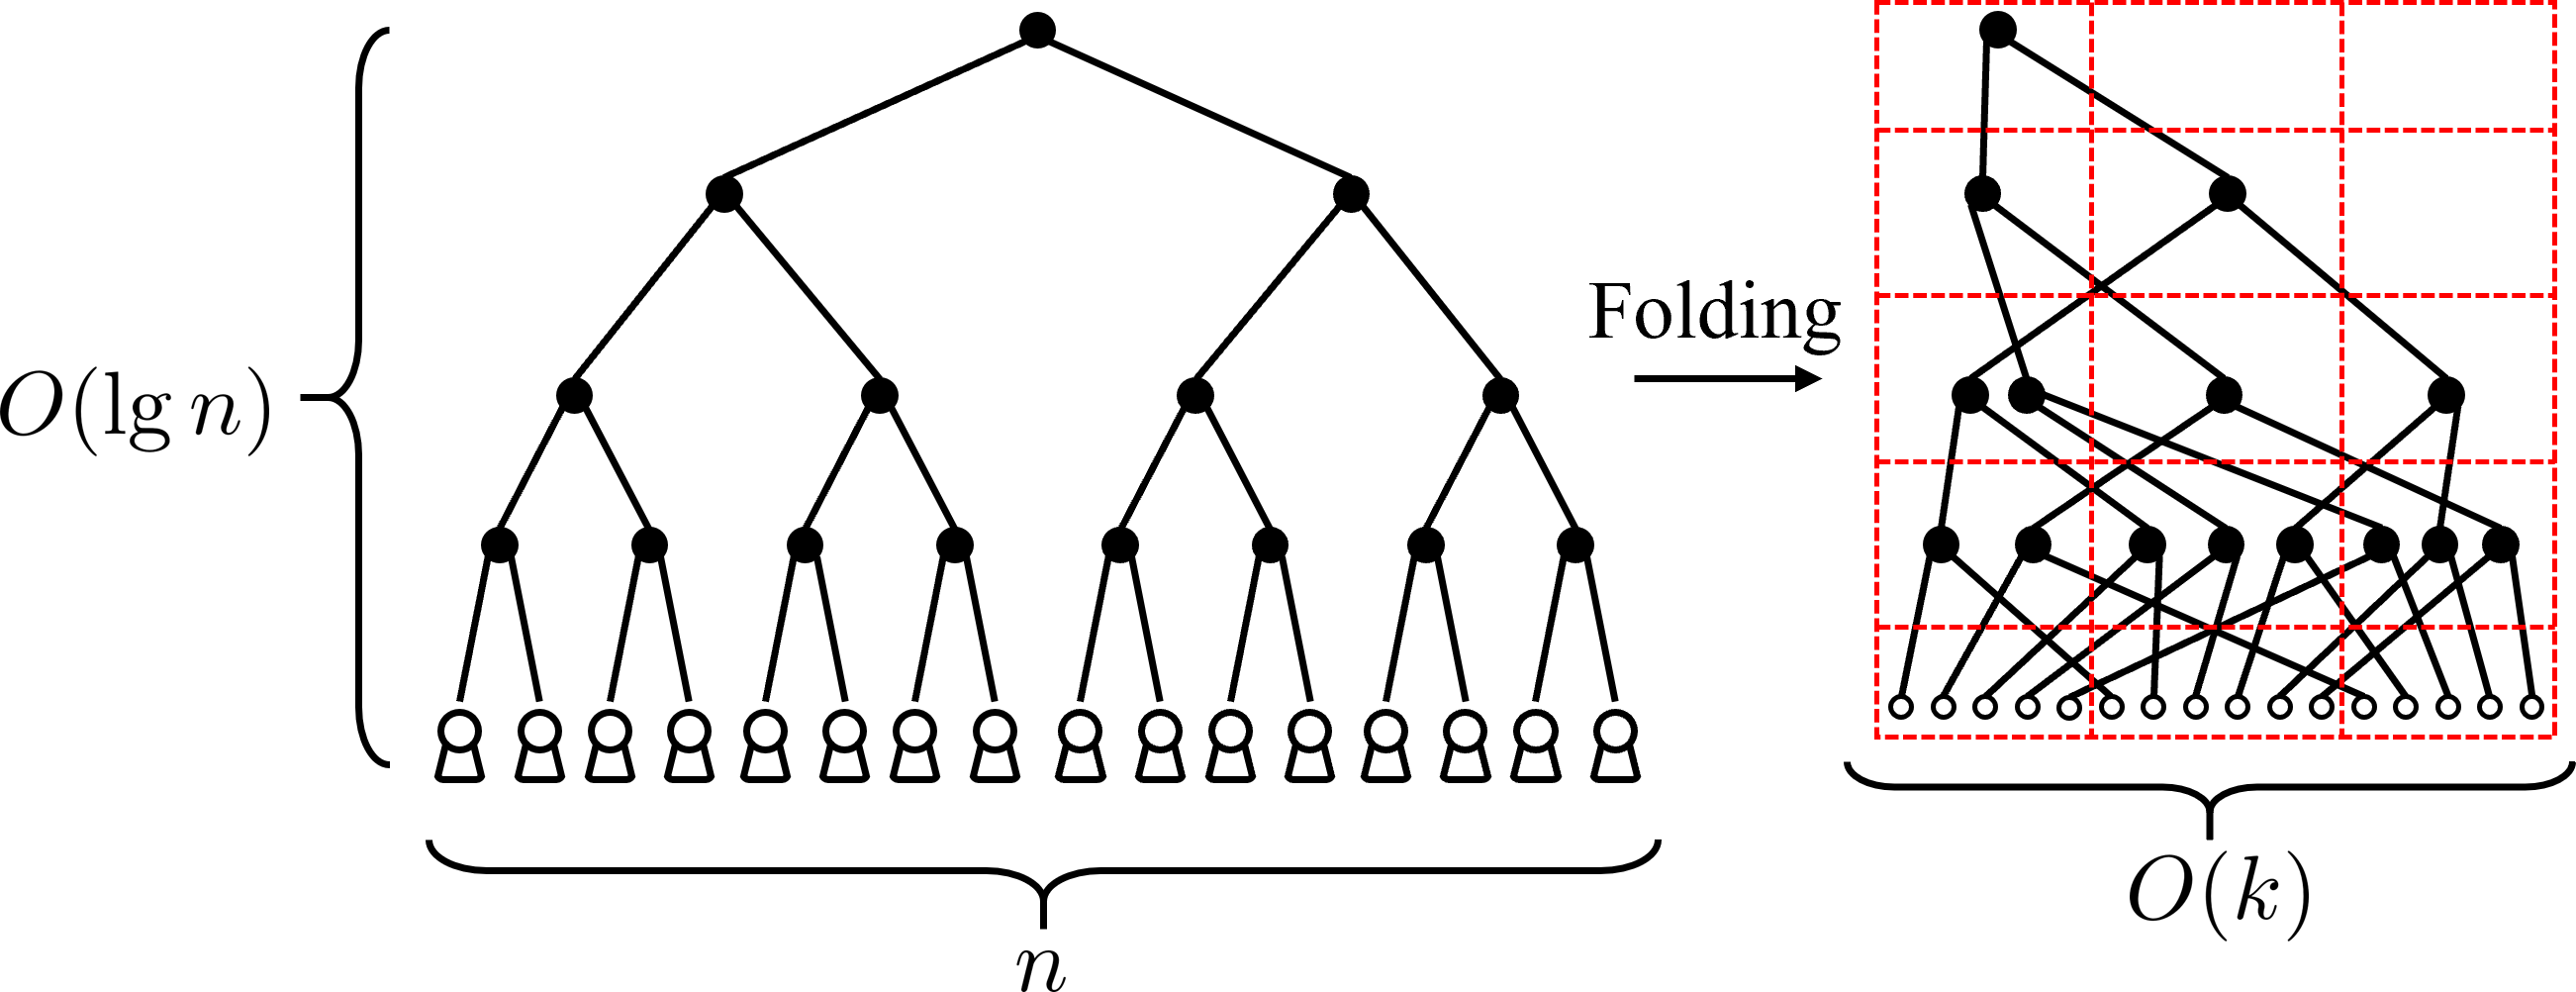
\includegraphics[width=0.8\linewidth]{figures/w12_bin_tree_GT.png}
    \caption{Binary search for group testing. The amount of tests required can be greatly reduced by folding the tree.}
    \label{fig:w12_bin_tree_GT}
\end{figure}

Normally, a non-adaptive group testing on a binary tree requires $O(n\lg n)$ tests. By simply folding the tree, however, one can devise a scheme that requires only $O(k\lg n)$ tests, this is also the information theoretical limit. See \autoref{fig:w12_bin_tree_GT}, each red box is a single test, testing all the leaves of the nodes within it. By pruning the tree with the negative tests, we should be able to find the infected population.

Tracing from the root to the leaves, one can construct a watch list $W$ of all the people suspected to be infected. For simplicity, let both $n$ and $k$ be a power of two, then each person is labeled by a bit string in $\{0,1\}^{\lg n}$. For each layer $j$, $W_j$ contains the prefixes of the $k$ sick people and with some healthy people that are still suspicious 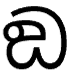
\includegraphics[height=1em]{figures/w12_sus.png}. At the first layer (the root), we have $W_1 = \{0,1\}$ since the test on the root must be positive ($k>0$). Then, on the second layer, $W_2 = \setdef{a0,a1}{a\in W_1, a \text{ is in a positive test}}$. Continue on, we have
\begin{equation}
    W_{j+1} = \setdef{a0,a1}{a\in W_j, a \text{ is in a positive test}}.
\end{equation}
At each level, we use $16k$ tests (so that the width to the right figure of \autoref{fig:w12_bin_tree_GT} is $16k=O(k)$). Let $w_j = \abs{W_j}$, 
\begin{equation}
    w_{j+1} = k + \mathrm{Ber}\left(2(w_j-k),\frac{1}{16}\right),
\end{equation}
where the probability $\frac{1}{16}$ is due to the fact that: there are $16k$ tests each layer, and there are $k$ infected person, the probability that each prefix contains no infected person will be pruned away is $15/16$.

\begin{definition}[Probability Generating Function]
    For a discrete random variable $X$ defined on non-negative integers, its probability generating function is defined as
    \begin{equation}
        F_X(x) = \sum_{\ell=0}^{\infty} \mathrm{Pr}\{X=\ell\} x^\ell.
    \end{equation}
\end{definition}
To facilitate discussion, let us define the \textit{excess size} of the watch list as $N_j \defeq w_j-k$ and $F_j = F_{N_j}$. We will also assume that each prefix of length $\lg k$ contains exactly one infected person, then
\begin{align}
    F_{\lg k}(x) &= 1, \\
    F_{j+1}(x) &= F_{j}\left(\frac{15}{16} + \frac{x^2}{16}\right) \cdot x^k. \label{eq:w12_branching}
\end{align}
\autoref{eq:w12_branching} defines a branching process, where with probability $\frac{15}{16}$ a suspicious prefix proves to be innocent, but with probability $\frac{1}{16}$ the number of suspected prefixes doubles. The term $x^k$ means that the $k$ infected people will each result in an innocent prefix.

Let us study the evolution of $F_j$. Define $f(x) = \frac{15}{16} + \frac{x^2}{16}$, such that
\begin{equation}
    F_{j+1}(x) = x^k \cdot f^k(x) \cdot \left(f^{\circ2}(x)\right)^k \cdot \left(f^{\circ3}(x)\right)^k \cdot \cdots \cdot \left(f^{\circ j}(x)\right)^k.
\end{equation}
The function $f$ is not entirely easy to iterate, hence we consider using a M\"obius transform $g$ to approximate it:
\begin{equation}
    g(x) \defeq \frac{6}{y-x} = f(x) + \underbrace{\frac{(x-1)(x-3)^2}{16(7-x)}}_{>0 \text{ for }x\in(1,6)}.
\end{equation}
Then
\begin{equation}
    g^{\circ j}(x) = 1 + \frac{5(x-1)}{6^j(6-x) + (x-1)},
\end{equation}
in particular $g^{\circ j}(5) \approx 1 + \frac{1}{6^j}$. Hence, we can bound $F_j$ by
\begin{equation*}
    F_j(5) \le \prod_{i=0}^{j} g^{\circ i}(5)^k \le \prod_{i=0}^{j} \left(1 + \frac{20}{6^i+4}\right)^k \le \prod_{i=0}^{j}\exp\left(\frac{20}{6^i+4}\right)^k \le \exp(7k).
\end{equation*}
Then we can bound $w_j$ by using the Chernoff bound:
\begin{equation*}
    \mathrm{Pr}\{w_j-k \ge 5k\} \le \frac{F_j(5)}{5^{5k}} \le \ee^{-k}.
\end{equation*}
With high probability, we have $\abs{W_j}\le 6k$. Our next goal will be to reduce the $6k$ down to $k$. Which can be done by random testing on these $6k$ people. Those $5k$ people that are innocent will quickly be found out.

Now that we have controlled $\abs{W_j}$, we are not satisfied, yet. We also want to control
\begin{equation*}
    \abs{W_1} + \abs{W_2} + \abs{W_3} + \cdots.
\end{equation*}
This is the idea of \textit{total progeny}: the sum of all the population from past to present. Our discussion is further aided by the following result.
\begin{theorem}[Dwass] \label{thm:w12_Dwass}
    Let the total progeny of 
\end{theorem}

\begin{remark}
    The original proof to \autoref{thm:w12_Dwass} is given by complex analysis. As a simple exercise, can you think of a combinatorial proof?
\end{remark}